\documentclass[11pt]{article}

\usepackage[portuguese]{babel}
\usepackage{float}
\usepackage[a4paper, margin=2cm]{geometry}
\usepackage{graphicx}
\usepackage{hyperref}
\usepackage{setspace}

\chardef\_=`_

\title{\textbf{Trabalho Prático de Sistemas Operativos}}
\author{
    \begin{centering}
        \textbf{Grupo TPSO2}
    \end{centering} \\
    \begin{tabular}{ll}
        Humberto Gomes & A104448 \\
        José Lopes     & A104541 \\
        José Matos     & A100612
    \end{tabular}
}
\date{7 de maio de 2024}

\begin{document}

\onehalfspacing
\setlength{\parskip}{\baselineskip}
\setlength{\parindent}{0pt}
\def\arraystretch{1.5}

\maketitle

\begin{abstract}
    % TODO
\end{abstract}

\section{Arquitetura multiprocesso}

O servidor desenvolvido utiliza uma arquitetura multiprocesso para ser capaz de correr várias
tarefas em simultâneo, tal como pedido pelo enunciado. O processo principal, o orquestrador, é
responsável por criar e coordenar outros processos. O modo como o servidor responde a mensagens do
cliente criando novos processos é descrito nesta secção. As mensagens mencionadas aqui são descritas
detalhadamente em anexo, na especificação do protocolo utilizado.

Quando o cliente pede a execução de uma nova tarefa através de uma escrita num \emph{pipe} com nome,
o orquestrador é responsável pelo seu \emph{parsing}, devolvendo ao cliente uma mensagem de sucesso
(\texttt{S2C\_TASK\_ID}) ou de erro (\texttt{S2C\_ERROR}). Na figura abaixo, pode observar-se o caso
em que o utilizador pede ao servidor a execução de um programa único (tipo de mensagem
\texttt{C2S\_SEND\_PROGRAM}), mas envia-lhe uma \emph{pipeline} (que deveria estar presente numa
mensagem \texttt{C2S\_SEND\_TASK}), resultando num erro de \emph{parsing} comunicado por um outro
\emph{pipe} com nome, exclusivo à instância do cliente.

\begin{figure}[H]
    \centering
    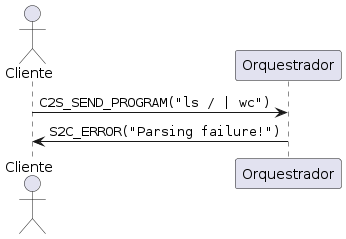
\includegraphics[width=0.4\textwidth]{report_figures/CommunicationParsingFailure.png}
    \caption{Comunicação entre o cliente e o servidor em caso de falha de \emph{parsing}.}
\end{figure}

No final de cada conexão, o servidor verifica se tem capacidade para a execução de mais tarefas e,
em caso afirmativo, cria um novo processo para a tarefa na frente da fila de espera. Este processo é
responsável por executar os vários programas presentes na tarefa (que pode ser uma \emph{pipeline}),
esperar pelo seu término, e avisar o orquestrador que ele mesmo terminou, através de uma escrita no
mesmo FIFO que o cliente utiliza (mensagem \texttt{C2S\_TASK\_DONE}). Deste modo, o orquestrador
sabe que pode executar a \emph{system call} bloqueante \texttt{wait()}. Na figura abaixo, observa-se
a receção e escalonamento imediato da primeira tarefa recebida pelo servidor:

\begin{figure}[H]
    \centering
    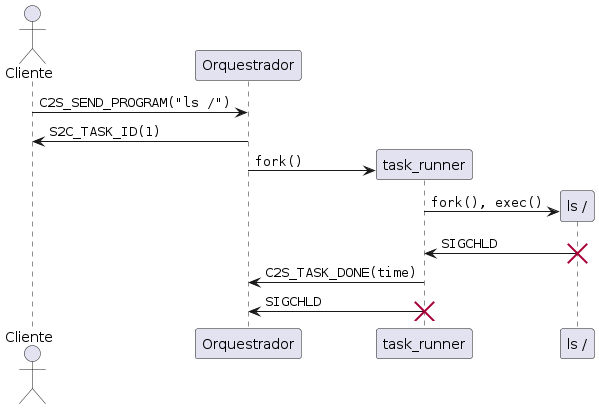
\includegraphics[width=0.65\textwidth]{report_figures/CommunicationSchedule.png}
    \caption{Comunicação entre o cliente e o servidor no caso da tarefa ser imediatamente
        escalonada.}
\end{figure}

O outro tipo de comunicação possível é um pedido de estado do servidor feito pelo cliente
(\texttt{C2S\_STATUS}). Como, para respeitar o que foi pedido pelo enunciado, o orquestrador não
deve parar de ler pedidos de utilizadores enquanto comunica o seu estado a outro, a comunicação de
estado ao cliente é feita por um processo distinto, como se vê na figura abaixo:

\begin{figure}[H]
    \centering
    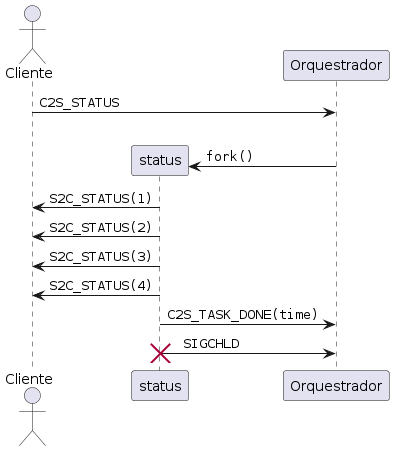
\includegraphics[width=0.4\textwidth]{report_figures/CommunicationStatus.png}
    \caption{Comunicação entre o cliente e o servidor num pedido de estado bem sucedido.}
\end{figure}

O processo de comunicação de estado transmite ao cliente, em mensagens \texttt{S2C\_STATUS}, as
várias tarefas em execução, em fila de espera e já executadas (estas últimas são lidas do histórico
do servidor guardado em ficheiro). Tal como ocorre com a execução de tarefas regulares, é
necessário informar o orquestrador que pode aguardar pelo processo filho quase a
\emph{zombieficar-se}. Como as tarefas de estado são escalonadas do mesmo modo que as tarefas
regulares, existe um limite superior de tarefas executadas em simultâneo. No entanto, para não se
fazer o cliente aguardar quando não há capacidade de escalonamento disponível, é enviada uma
mensagem de erro, como se vê na figura abaixo:

\begin{figure}[H]
    \centering
    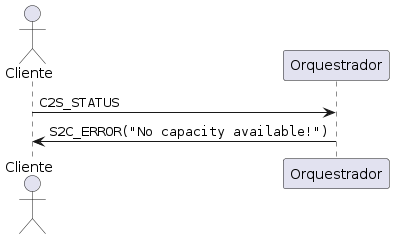
\includegraphics[width=0.4\textwidth]{report_figures/CommunicationStatusFailure.png}
    \caption{Comunicação entre o cliente e o servidor num pedido de estado falhado.}
\end{figure}

\section{Arquitetura modular}

A arquitetura do \emph{software} desenvolvido pode ser abordada de diversas perspetivas, tal como a
da organização do código em diversos módulos, vistos na figura abaixo: \\

\begin{figure}[H]
    \centering
    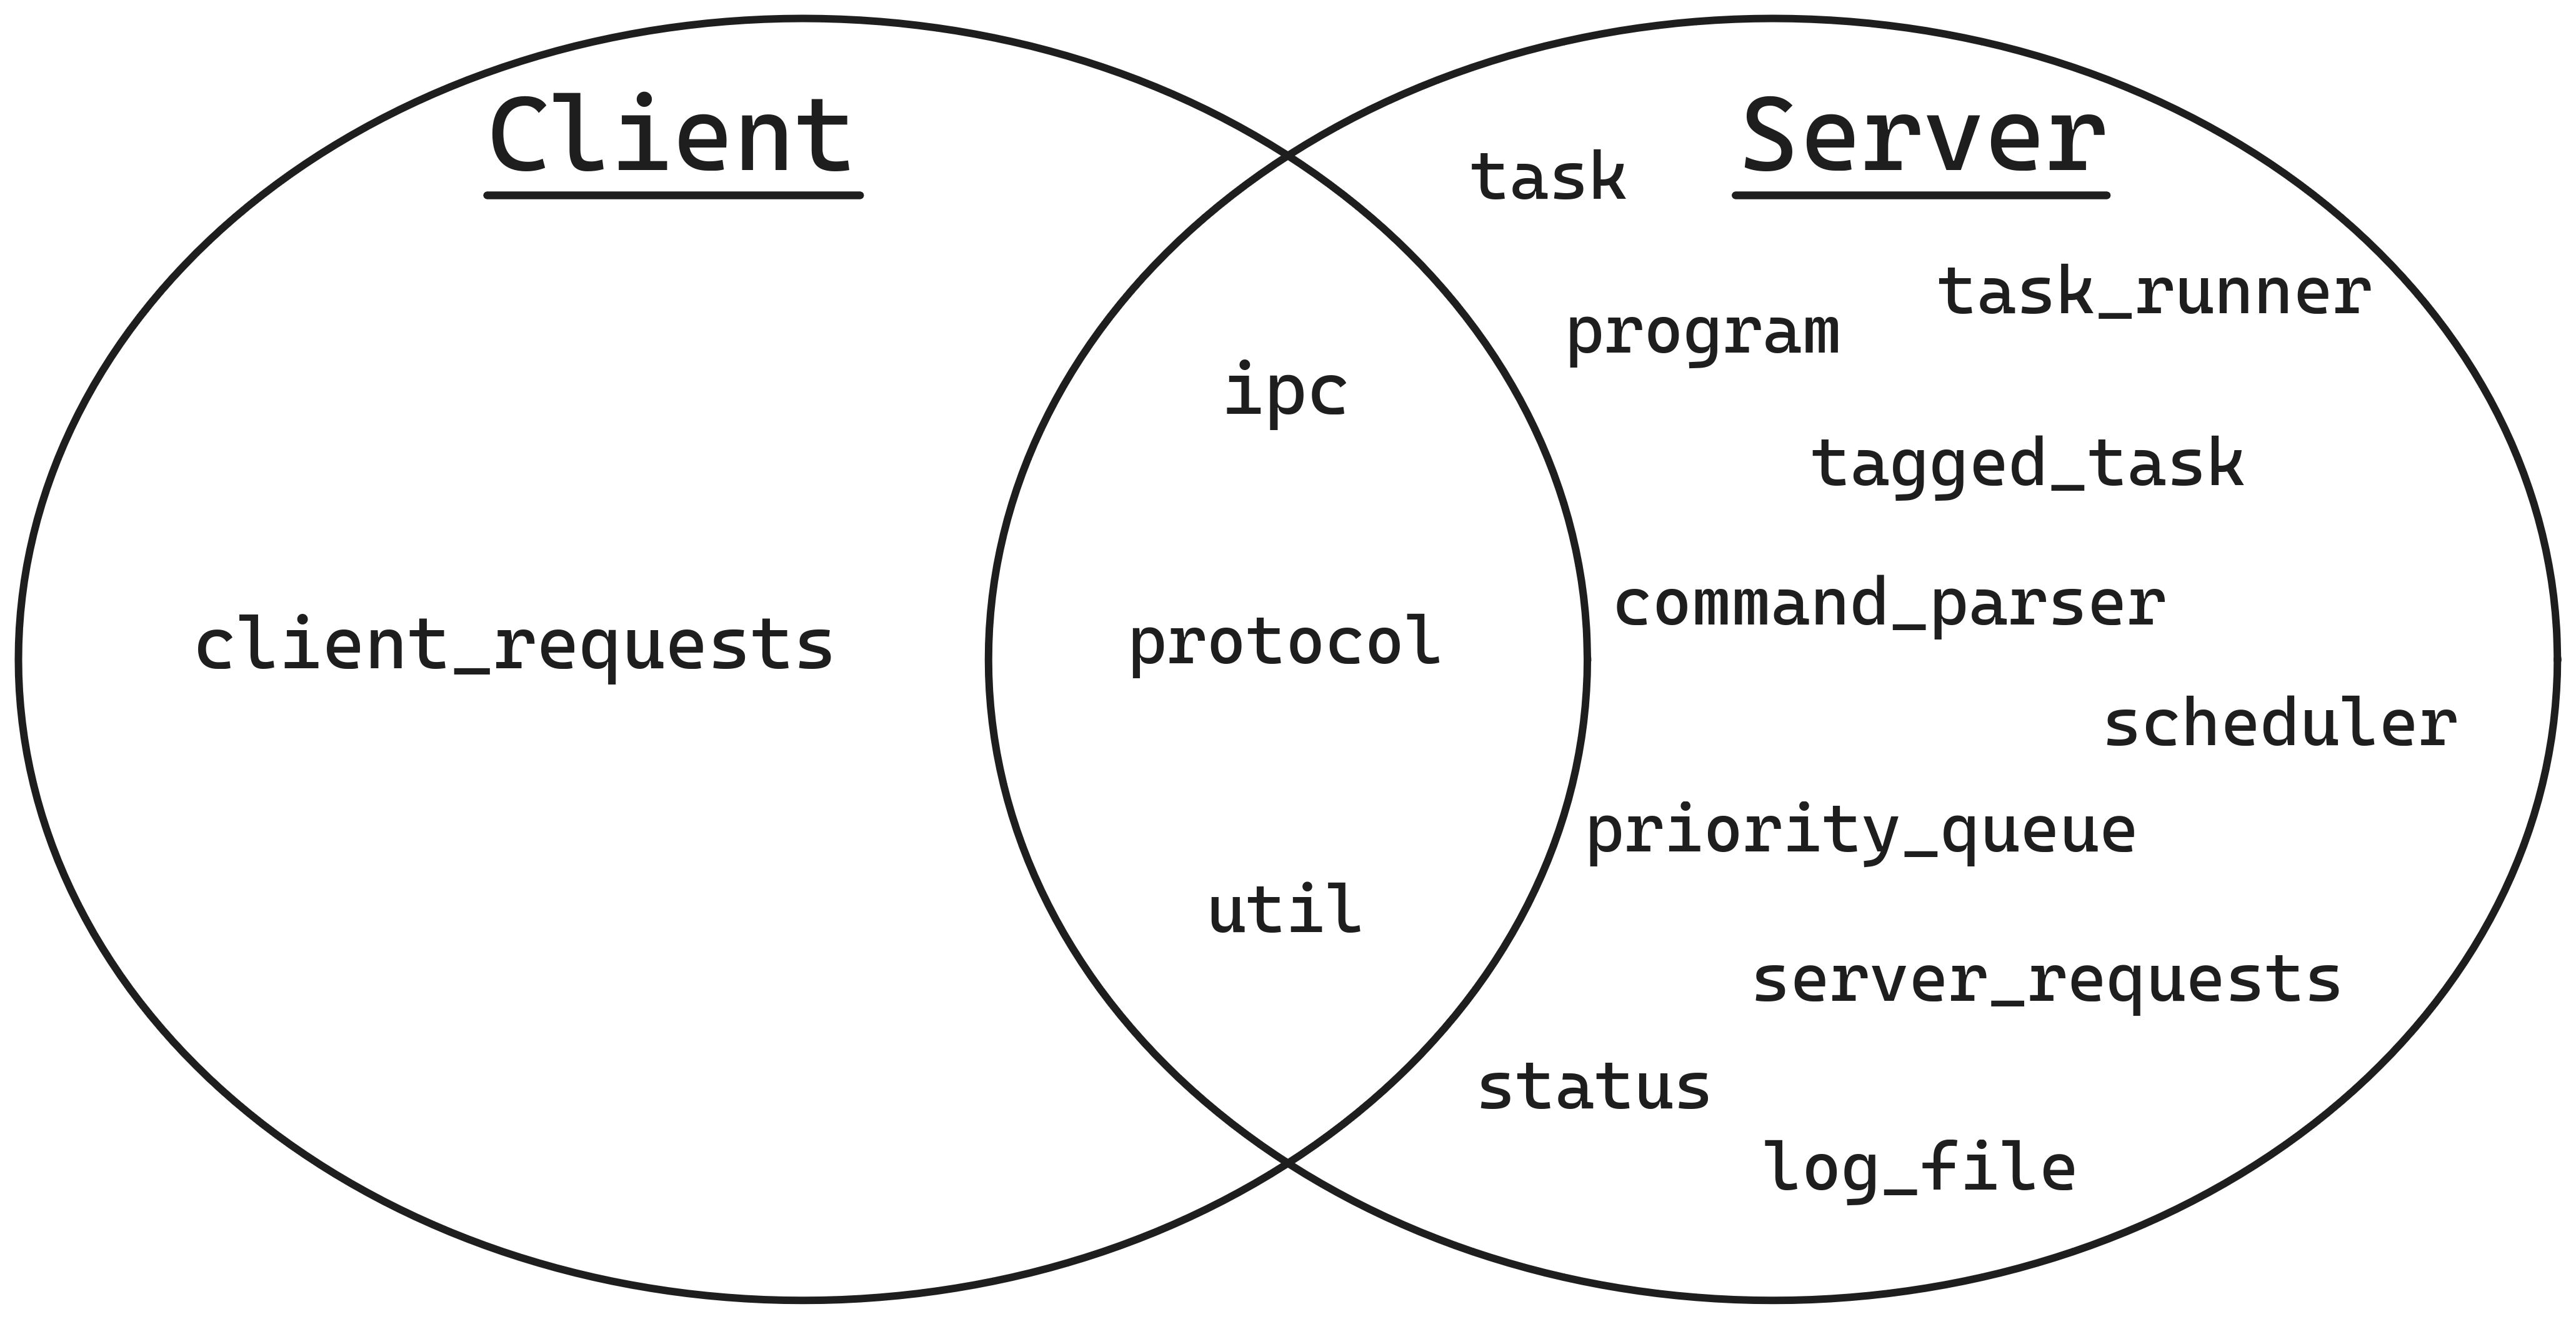
\includegraphics[width=0.6\textwidth]{report_figures/modules_venn_diagram.png}
    \caption{Módulos presentes no cliente e no servidor.}
\end{figure}

Alguns módulos são partilhados pelo cliente e pelo servidor: \texttt{util} fornece utilidades de
escrita para \texttt{stdout} e \texttt{stderr} utilizando a \emph{system call} \texttt{write};
\texttt{ipc} é responsável pela comunicação interprocesso a um nível mais básico (abertura de
conexões e separação de mensagens) utilizando \emph{pipes} com nome, enquanto que em
\texttt{protocol} estão definidas as estruturas das mensagens serializadas, transmitidas entre o
cliente e o servidor, e vice-versa.

O único módulo presente apenas no cliente é \texttt{client\_requests}, que é responsável por enviar
mensagens ao servidor e receber as suas respostas. No servidor, o módulo \texttt{server\_requests}
tem o papel dual: espera por pedidos do cliente para lhes responder. Este módulo é também
responsável por coordenar, conforme as mensagens que são recebidas, as escritas para o ficheiro de
\emph{logs}, feitas pelo módulo \texttt{log\_file}.

Há várias estruturas de dados no servidor. \texttt{program} é um \emph{array} de argumentos
terminado em \texttt{NULL}, facilmente providenciado a uma função na família \texttt{exec}. Vários
programas formam uma \emph{pipeline} em \texttt{task}, que alternativamente pode ser constituída por
um procedimento de C (é possível escalonar tarefas que não programas independentes). Há mais
informação necessária para a gestão de tarefas do que uma lista de programas, como identificadores e
tempos em filas de espera. Uma \texttt{tagged\_task} é formada por uma \texttt{task} e por esta
informação. Continuando-se a cadeia de composição, tem-se a estrutura \texttt{priority\_queue}, uma
\emph{minheap} de tarefas, onde definir uma política de escalonamento se torna tão simples como
definir uma função de comparação entre tarefas.

Vários outros módulos são responsáveis pela funcionalidade do servidor. Apesar de uma \texttt{task}
poder ser criada manualmente, programa a programa, a funcionalidade de interpretação de uma
\emph{string} de linha de comandos é providenciada pelo módulo \texttt{command\_parser}. Tivemos o
cuidado de que este módulo suportasse aspas únicas e duplas corretamente. Um outro módulo é
\texttt{scheduler}, responsável por saber que tarefas estão em execução e em fila de espera, criando
novos processos para a execução de novas tarefas desde que tenha disponibilidade para tal. Há dois
programas que são executados, \texttt{status}, responsável por enviar ao cliente informação sobre o
servidor sem o bloquear, e \texttt{task\_runner}, responsável pela execução de tarefas como
\emph{pipelines}, informando o seu processo pai quando estas terminam.

A arquitetura modular utilizada foi essencial para o \emph{software} desenvolvido. Não só garante
código de melhor qualidade, como permite evitar erros (como erros de memória e invariantes violadas)
que ocorrem devido à quebra do encapsulamento. A manutenção do código também se tornou mais simples.
Por exemplo, foi necessária, devido a um \emph{bug} que não se conseguiu resolver, a mudança
completa do protocolo definido em \texttt{ipc.c}. Foi possível reescrever este ficheiro mantendo a
interface das funções nele definidas, e o servidor manteve-se operacional sem qualquer outra mudança
necessária.

\section{Testes executados}

Foram escritos testes para avaliar diversos aspetos do \emph{software} desenvolvido, tanto de um
ponto de vista funcional como de desempenho. Nesta secção são descritos os testes desenvolvidos e
as correções que deles resultaram.

O teste \texttt{fds.sh} verifica quais são os descritores de ficheiro abertos num processo criado
pelo servidor em qualquer posição possível numa \emph{pipeline}. Em princípio, o descritor 0
(\texttt{stdin}) devia estar aberto para todos os processos que não o primeiro da \emph{pipeline}, e
os descritores 1 e 2 (\texttt{stdout} e \texttt{stderr}) deveriam ser os únicos restantes abertos
para qualquer processo. No entanto, outros descritores abertos foram detetados e o código de
\texttt{task\_runner} foi corrigido para fechar alguns descritores de \emph{pipes} que se mantinham
abertos. Este é o único teste que não corre em outros sistemas POSIX que não Linux, pois precisa de
acesso à diretoria \texttt{/proc/self/fd}.

De seguida, o teste \texttt{length.sh} verifica que o servidor suporta corretamente mensagens com o
comprimento máximo especificado, necessário para garantir a atomicidade de escritas no FIFO.
Inicialmente, tarefas com comandos muito longos podiam ser escalonadas, mas não surgiam num pedido
de \texttt{status} do cliente. Caso o comprimento do comando de uma tarefa seja superior ao
permitido por uma mensagem de estado, o comando é substituído pela \emph{string}
\texttt{"COMMAND TOO LONG"}.

O teste \texttt{order.sh} garante que os processos enviados ao servidor são escalonados corretamente
conforme a política de escalonamento definida. Este teste não revelou qualquer erro no comportamento
do servidor. Outro teste que não revelou problemas foi \texttt{parser.sh}, que garante que o
\emph{parser} de linhas de comando funciona como esperado. Outro teste que não exigiu alterações ao
código escrito foi \texttt{pipelines.sh}, que testa se os \emph{pipes} entre comandos são capazes de
transmitir mais informação do que a sua capacidade. Fá-lo através da transferência de um vídeo do
YouTube, aplicando efeitos ao seu áudio, e reproduzindo-o, sem alguma vez escrever para o sistema de
ficheiros.

Ademais, o teste \texttt{status.sh} procura verificar se o servidor consegue enviar o seu estado ao
cliente corretamente. Detetou-se perda de mensagens quando em elevadíssimo número, erro cuja causa
não se conseguiu descobrir, levando a que o módulo \texttt{ipc} fosse reescrito para deixar de usar
mensagens de comprimento variável, passando a utilizar mensagens de comprimento fixo.

De seguida, \texttt{stress.sh} cria milhares de processos de clientes, que tentam comunicar com o
servidor em simultâneo pelo FIFO partilhado. Detetou-se a possibilidade do servidor fechar o seu
descritor durante a escrita de um cliente, resultando na terminação deste com um \texttt{SIGPIPE}.
Não é um grande problema o cliente falhar, mas esta falha de comunicação pode ocorrer quando um
processo filho do orquestrador tenta avisar o seu pai que a sua execução está prestes a terminar.
Se o servidor não receber esta mensagem, nunca saberá que um dos seus filhos terminou e que passa a
ter mais capacidade de escalonamento disponível. Foi-nos permitido, pelo regente da UC, ignorar o
sinal através da \emph{system call} \texttt{signal}, permitindo que \texttt{write} termine com um
código de erro, podendo retentar-se a comunicação com o servidor.

Por último, o ficheiro \texttt{benchmark.sh} procura analisar o desempenho das políticas de
escalonamento \emph{First Come First Served} (FCFS) e \emph{Shortest Job First} (SJF), fazendo
pedidos de cem tarefas de duração entre 300 milissegundos e 2 segundos. No final, o estado do
servidor é requisitado, revelando informação sobre o tempo de espera e de execução das tarefas, que
sofre uma conversão para um formato CSV, importado para uma folha de cálculo e analisado:

\begin{figure}[H]
    \centering
    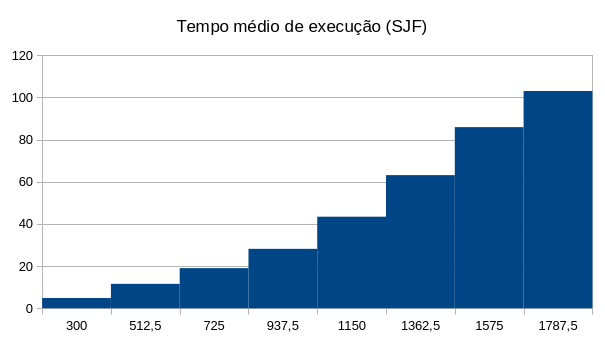
\includegraphics[width=0.45\textwidth]{report_figures/HistogramSJF.png}
    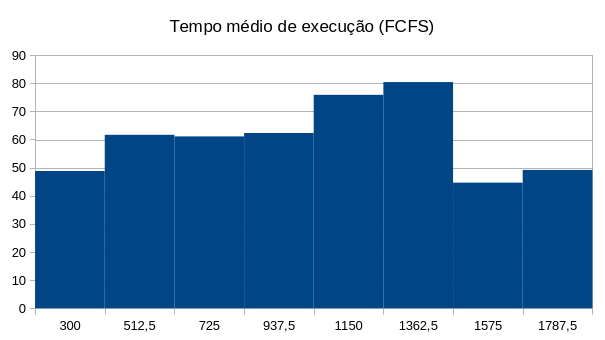
\includegraphics[width=0.45\textwidth]{report_figures/HistogramFCFS.png}
    \caption{Tempos médios de execução de tarefas (desde o cliente até o fim da execução, em
        segundos) em função da sua duração (em milissegundos), agrupada em oito conjuntos, conforme
        a política de escalonamento usada.}
\end{figure}

\begin{figure}[H]
    \centering
    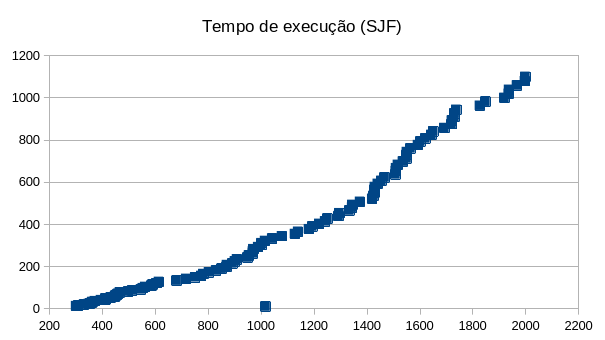
\includegraphics[width=0.45\textwidth]{report_figures/ScatterSJF.png}
    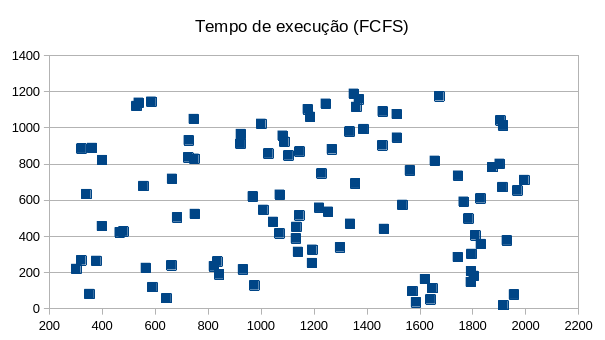
\includegraphics[width=0.45\textwidth]{report_figures/ScatterFCFS.png}
    \caption{Tempos de execução de tarefas (desde o cliente até o fim da execução, em segundos) em
        função da sua duração (em milissegundos), conforme a política de escalonamento usada.}
\end{figure}

Conforme esperado, quando a política SJF é utilizada, tarefas de menor duração passam menos tempo em
fila de espera (a maior contribuição para o tempo total de execução) do que as tarefas mais longas,
evidenciado pelo comportamento crescente tanto no histograma como no \emph{scatter}. Por outro lado,
o tempo de execução quando se aplica a política FCFS é relativamente uniforme, evidenciado pela
altura relativamente próxima das barras do histograma e da aleatoriedade no \emph{scatter}.

Como na política SJF as tarefas mais rápidas são executadas em primeiro lugar, os tempos de espera
das primeiras tarefas são muito baixos, reduzindo o tempo médio de espera total. Esta tese
verifica-se: SFJ apresenta um tempo médio de espera de 402 segundos mas estes tornam-se 592 segundos
para FCFS. No entanto, em FCFS, tarefas de maior duração experienciam menor tempo médio, como se
observa no primeiro par de gráficos. Logo, a escolha de uma política de escalonamento depende do
tipo de tarefa que se pretende valorizar: usa-se SJF para processos de curta ou média duração, e
FCFS para tarefas mais longas.

\section{Decisões relevantes}

Nesta secção, são discutidas algumas decisões tomadas ao longo do desenvolvimento do projeto que o
nosso grupo julga serem relevantes de se mencionar.

Inicialmente, o nosso grupo pensava em fazer um orquestrador seguro, capaz de estar presente num
sistema partilhado (\emph{multiseat}). No entanto, foi rápida a conclusão de que sem virtualização
(ou \emph{containerização}) seria possível um cliente enviar uma tarefa como \texttt{pkill
orchestrator}. Ademais, poderiam ser envidas várias tarefas sem fim, tirando toda a capacidade ao
servidor, sem que este as possa matar devido à proibição de se utilizarem sinais. Logo, o objetivo
de segurança foi descartado e o foco do grupo passou para a robustez do servidor, que foi programado
de modo a resistir a erros tanto internos (como \emph{system calls} falhadas) como externos
(mensagens mal formatadas no FIFO), procurando recuperar e voltar a um estado conhecido. Ademais,
durante o desenvolvimento, foi sendo executado o \texttt{valgrind} \cite{valgrind} para procurar
erros de memória como acessos indevidos e \emph{leaks}. Após os vários testes realizados e falhas
propositadamente provocadas, julgamos que o servidor seja capaz de continuar a operar corretamente
sem \emph{crashes}.

Ademais, o nosso grupo optou por utilizar uma \emph{minheap} (\texttt{priority\_queue}) para as
políticas de escalonamento SJF e FCFS, apesar de tal não conduzir ao melhor desempenho.
\emph{Minheaps} apresentam complexidades (caso médio) de $\Theta(1)$ para inserção e
$\Theta(\log n)$ para remoção. Estas são ideais para SJF, mas seria possível uma remoção em tempo
constante para FCFS caso se utilizasse uma fila simples. No entanto, por motivos de simplicidade,
preferiu-se o uso de uma única estrutura de dados com pior desempenho do que a adição de código
necessária para se suportarem duas estruturas.

Além disso, deve ser mencionado que apenas foram usadas as bibliotecas \texttt{libc}, \texttt{libm}
e \texttt{librt}, todas constituintes da biblioteca POSIX de C. Não foi utilizado código de
terceiros para a implementação de estruturas de dados, dado que quando a equipa docente publicou a
FAQ a explicitamente autorizar o seu uso, já as estruturas de dados como \emph{arrays} dinâmicos e
filas de prioridade tinham sido implementadas pelo nosso grupo.

Por último, é importante mencionar que fomos contra a recomendação do enunciado de utilizar a
\emph{system call} \texttt{gettimeofday} para a medição de intervalos temporais, utilizando
\texttt{clock\_gettime} no seu lugar. \texttt{gettimeofday} é uma função depreciada desde 2008
\cite{gettimeofday}, sendo que a sua substituição, \texttt{clock\_gettime}, já foi introduzida em
2001, pelo que o seu uso não afetaria significativamente a portabilidade do \emph{software}
desenvolvido. Ademais, esta função, quando usada com \texttt{CLOCK\_MONOTONIC}, não é influenciada
por mudanças no relógio do computador (por exemplo, um ajuste do utilizador), garantindo sempre que
o valor de tempo devolvido aumenta e que não se calculam intervalos de tempo negativos.
\cite{clock_gettime}

\section{Conclusão}

Após a conclusão deste trabalho prático, há vários aspetos do produto final que podem ser
discutidos. Em primeiro lugar, o nosso grupo julga ter cumprido com correção os objetivos
estipulados pelo enunciado. Ademais, encontra-se satisfeito com a qualidade do código escrito:
contribuem para a sua facilidade de compreensão, modificação e extensão não só a farta documentação
como também a estrutura modular.

No entanto, sentiram-se algumas dificuldades que prejudicaram a qualidade do \emph{software}
produzido. Em primeiro lugar, uma parte considerável do código dedica-se à resiliência a erros e à
serialização de mensagens. Este código apresenta bastante verbosidade, distraindo o seu leitor da
verdadeira funcionalidade de cada procedimento. Uma possível solução para este problema seria o uso
de uma linguagem de programação que não exija muita verbosidade para estas tarefas, mas permita, tal
como C, controlo direto sobre a interação com o sistema operativo. Por exemplo, Zig encaixa-se
nestes critérios e o nosso grupo julga que seja uma linguagem ideal para o projeto de SO.

Ademais, devido à natureza dos descritores de ficheiros em sistemas UNIX, foi difícil conservar uma
boa arquitetura modular. Como são duplicados para processos filhos, foi frequente a necessidade de
estes fecharem os descritores, mas tal complexifica as relações de dependência entre módulos, dado
que os processos criados precisam de conhecer todas as estruturas de dados com descritores abertos.
Se o \emph{standard} POSIX definisse uma \emph{flag} semelhante a \texttt{O\_CLOEXEC} mas para a
\emph{system call} \texttt{fork()}, não teríamos este problema.

Logo, considerando as limitações com que tivemos de lidar, o nosso grupo considera ter desenvolvido
uma solução de qualidade para o problema proposto pelo enunciado. No entanto, caso fosse permitido o
uso de sinais, poder-se-ia desenvolver um servidor completamente diferente, com suporte para
políticas de escalonamento com desafetação forçada, \emph{timeouts} para assegurar uma maior
proteção contra ataques \emph{Denial of Service} e muitas outras funcionalidades, apesar de tal
exigir uma arquitetura muito distinta.

% Isto é uma grande gambiarra, mas funciona para pôr a bibliografia como uma secção.
\section{Bibliografia}
\def\refname{}
\vspace{-1.5cm}
\begin{thebibliography}{9}
    \bibitem{valgrind}
         Valgrind Developers, "Valgrind". valgrind.org.
         \url{https://valgrind.org/}
         (accessed May 4, 2024).
    \bibitem{gettimeofday}
        IEEE and The Open Group, "The Open Group Base Specifications Issue 7, 2018 edition".
        pubs.opengroup.org
        \url{https://pubs.opengroup.org/onlinepubs/9699919799/functions/gettimeofday.html}
        (accessed May 4, 2024).
    \bibitem{clock_gettime}
        IEEE and The Open Group, "The Open Group Base Specifications Issue 7, 2018 edition".
        pubs.opengroup.org
        \url{https://pubs.opengroup.org/onlinepubs/9699919799/functions/clock_gettime.html}
        (accessed May 4, 2024).
\end{thebibliography}

\end{document}
